% Very simple template for lab reports. Most common packages are already included.
\documentclass[a4paper, 11pt]{article}
\usepackage[utf8]{inputenc} % Change according your file encoding
\usepackage{graphicx}
\usepackage{url}
\usepackage{fancyvrb}

%opening
\title{Groupy: a group membership service}
\author{Chrysoula Dikonimaki}
\date{\today{}}

\begin{document}
\maketitle

\section{Introduction}
The goal of this exercise was to implement Groupy, a group membership service that provides atomic multicast. Atomic multicast means that all nodes will receive the message at the same order, total order. 

\section{The Service}
Without calling the crash function, all nodes has the same color all the time and hopefully they will never stop working. But when we call the crash function we simulate nodes which crash so we should define the probability of crashing (arghh=100 means 1/100 will crash, arghh=10 means 1/10 etc). 

In Figure \ref{exp1} we can see the result of running the 3rd version of our service. We initialized 5 nodes. At the end, the first 4 nodes have crashed and only the last one was remaining alive.

\begin{figure}
  \begin{center}
    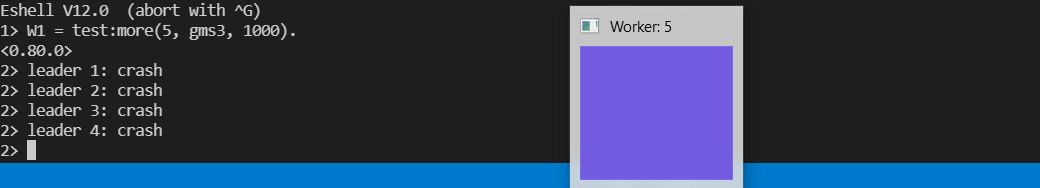
\includegraphics[scale=0.5]{exp1.PNG}
    \caption{Handling crashed nodes}
    \label{exp1}
  \end{center}
\end{figure}

\section{Optional task}
\subsection{Handling the possible lost messages}
I copied the third version of our service (gms3) at a file called gms4. I excluded from the code the crash function because I wanted to concentrate on the current task. 

First of all, I had to simulate the lost messages. I did it by not sending some messages at all with a specific probability (see macro pro). The code doing this is the send\_or\_not function. 

I chose to implement the idea I had only to the broadcast messages with the tag 'msg' sent from the Leader to the Clients. I could implement it to all messages but I just wanted to put emphasis on the algorithm and didn't want to make things too complex.

The idea that I implemented is the following: When we broadcast a message (in our case, the Leader) we create a unique reference for each one of these messages. After sending them, we are waiting for some secs (timeout2). When we receive an ACK (in our case, the Slaves send them) that the message has been sent we can delete from the list the reference of this message because this means that the other node has received it. 

If we have received the ACKs for all the messages, we can continue. On the other hand, if we haven't received an ACK message for each message after some time (we haven't received any message for a specific time) we will resend the messages that we haven't got an ACK for. When we resend the message we will keep the same reference for it, because if we received an old ACK, which might have been delayed, it's fine.

However, we don't want to try to resend the message forever (maybe a node has crashed and we haven't detected it) that's why I added an extra parameter called times, which will define the number of times we will try to resend the list of messages that we haven't received a reply from.

It would be interesting to change the parameters (prob, timeout2, prob) and see how the system works. Some results are shown below. There are some cases that some nodes won't receive the message on time or they won't receive it at all, for example if the message was being lost again and again until times parameter became 0. We can see an example in Figure \ref{exp2}.

The times parameter plays an important role when the prob parameter is low (which means that the probability of losing a message is high). When it happens, we need to set the times parameter to a high value as well if we want to reduce the probability of some nodes not getting some messages at all. The results of setting prob=10 and times=1 is shown in Figure \ref{exp3}. If we have such an unreliable system (low prob parameter) we will have to set times to a higher value if we want to avoid losing so much messages.

After trying some values for the parameters, if we had a system with prob=100, then times=4 seems to work fine.

\begin{figure}
  \begin{center}
    
\includegraphics[scale=0.3]{exp2.PNG}
    \caption{Handling lost messages: Lost message}
    \label{exp2}
  \end{center}
\end{figure}


\begin{figure}
  \begin{center}
    
\includegraphics[scale=0.3]{exp3.PNG}
    \caption{Handling lost messages: High probability of lost message}
    \label{exp3}
  \end{center}
\end{figure}

\subsection{Can we rely that the Erlang failure detector is perfect?}
When a process A monitors a process B, it means that if B fails A will receive a message of this failure. Practically, A has received a message that B has failed.
So even if the Erlang failure detector is perfect and can always determine when a node has failed there is always a chance of this message to be lost if our network is unreliable.


\section{Conclusions}
There are many things that can go wrong when we're developing distributed systems e.g. nodes are crashing, messages might be lost. We have to understand about those possible failures and try to handle them when it's possible. We may not achieve to handle them completely, but reducing the number of times they happen or hide them with some way will improve our system.
\end{document}
